\documentclass{beamer}
\usepackage[utf8]{inputenc}

\usetheme{Madrid}
\usecolortheme{default}
\usepackage{amsmath,amssymb,amsfonts,amsthm}
\usepackage{txfonts}
\usepackage{tkz-euclide}
\usepackage{listings}
\usepackage{adjustbox}
\usepackage{array}
\usepackage{tabularx}
\usepackage{gvv}
\usepackage{lmodern}
\usepackage{circuitikz}
\usepackage{tikz}
\usepackage{graphicx}
\usepackage{gensymb} % For using \degree symbol

\setbeamertemplate{page number in head/foot}[totalframenumber]

% Title Information
\title{2.7.15}
\date{September 30, 2025}
\author{ADHARVAN KSHATHRIYA BOMMAGANI - EE25BTECH11003}

\begin{document}

% Title Slide
\frame{\titlepage}

% Question Slide
\begin{frame}{Question}
Find the volume of a parallelepiped whose edges are given by:
\begin{align*}
\vec{a} = -3\hat{i} + 7\hat{j} + 5\hat{k}, \quad
\vec{b} = -5\hat{i} + 7\hat{j} - 3\hat{k}, \quad
\vec{c} = 7\hat{i} - 5\hat{j} - 3\hat{k}
\end{align*}
\end{frame}

% Vectors definition
\begin{frame}{Theoretical Solution}
Let $\vec{a}$, $\vec{b}$ and $\vec{c}$ be the vectors representing the edges of the parallelepiped:
\begin{align*}
\vec{a} &= \myvec{-3 \\ 7 \\ 5}, \\
\vec{b} &= \myvec{-5 \\ 7 \\ -3}, \\
\vec{c} &= \myvec{7 \\ -5 \\ -3}
\end{align*}
\end{frame}

% Volume definition using scalar triple product
\begin{frame}{Theoretical Solution}
The volume is given by the scalar triple product:
\begin{align*}
V = \left| [\vec{a} \ \vec{b} \ \vec{c}] \right|
\end{align*}
This is equivalent to the determinant:
\begin{align*}
V = \left| \myvec{ -3 & -5 & 7 \\ 7 & 7 & -5 \\ 5 & -3 & -3 } \right|
\end{align*}
\end{frame}

% Determinant calculation
\begin{frame}{Theoretical Solution}
Expanding the determinant:
\begin{align*}
\det 
&= -3(-21 - 15) + 5(-21 + 25) + 7(-21 - 35) \\
&= -3(-36) + 5(4) + 7(-56) \\
&= 108 + 20 - 392 = -264
\end{align*}
\end{frame}

% Final Volume
\begin{frame}{Theoretical Solution}
Taking the absolute value of the determinant:
\begin{align*}
V &= |{-264}| = 264 \text{ cubic units}
\end{align*}
Therefore, the volume of the parallelepiped is 264 cubic units.
\end{frame}

% Figure slide
\begin{frame}{Plot}
\centering
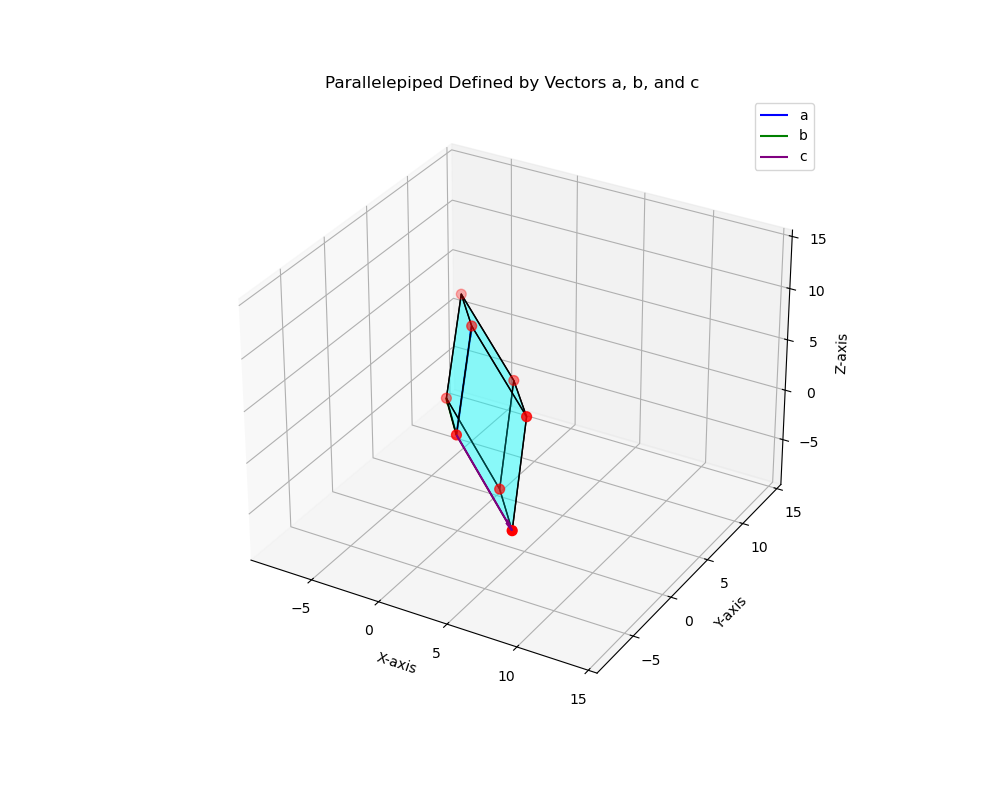
\includegraphics[width=0.8\linewidth]{figs/fig1.png}
\captionof{figure}{Parallelepiped Defined by Vectors $\vec{a}$, $\vec{b}$, and $\vec{c}$}
\end{frame}

\end{document}
